\noindent

\includegraphics[height=1.25cm]{images/pictograms/replication}

\includegraphics[height=1.25cm]{images/pictograms/benchmark}

\includegraphics[height=1.25cm]{images/pictograms/FEM}

\includegraphics[height=1.25cm]{images/pictograms/paraview}

%%%%%%%%%%%%%%%%%%%%%%%%%%%%%%%%%%%%%%%%%%%%%%%%%%%%%%%%%%%%%%%%%%%%%%%%%%%%%%%%%%%%%%%%%%%%%%%%%%%

%\lstinputlisting[language=bash,basicstyle=\small]{python_codes/fieldstone_06/keywords.ascii}

\begin{center}
\inpython
{\small Code at \url{https://github.com/cedrict/fieldstone/tree/master/python_codes/fieldstone_06}}
\end{center}

\par\noindent\rule{\textwidth}{0.4pt}

Last revision: August 30th, 2025.

\par\noindent\rule{\textwidth}{0.4pt}

%%%%%%%%%%%%%%%%%%%%%%%%%%%%%%%%%%%%%%%%%%%%%%%%%%%%%%%%%%%%%%%%%%%%%%%%%%%%%%%%%%%%%%%%%

The SolKz benchmark \cite{repa87} is similar to the SolCx benchmark.
but the viscosity is now a function of the space coordinates: 
\begin{equation}
\eta(y)=\exp(By) \quad {\rm with} \quad B=13.8155
\end{equation}
It is however not a discontinuous function but grows exponentially with the vertical coordinate so that its overall variation is again $10^6$. 
The forcing is again chosen by imposing a spatially variable density variation as follows:
\begin{equation}
\rho(x,y)=\sin(2y) \cos(3\pi x)
\end{equation}
Free slip boundary conditions are imposed on all sides of the domain.
This benchmark is presented in Zhong (1996) \cite{zhon96} as well and is studied 
in Duretz \etal (2011) \cite{dumg11} and Gerya \etal (2013) \cite{gemd13}.

Note that the matrx storage and imposition of boundary conditions is still 
of the naive type in the code. 

\begin{center}
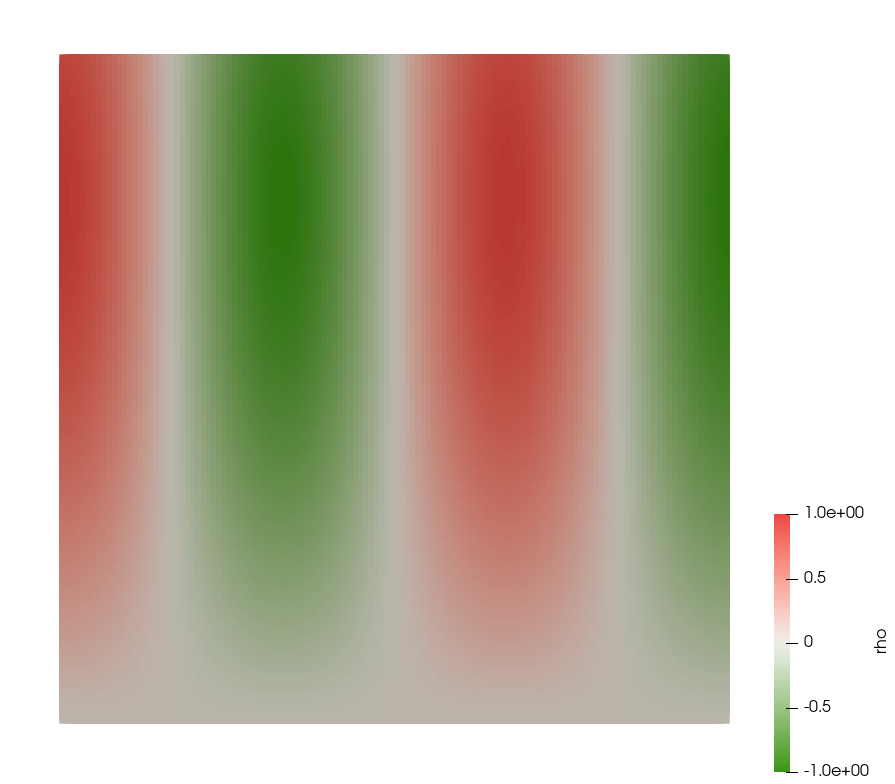
\includegraphics[width=6.5cm]{python_codes/fieldstone_06/results/rho}
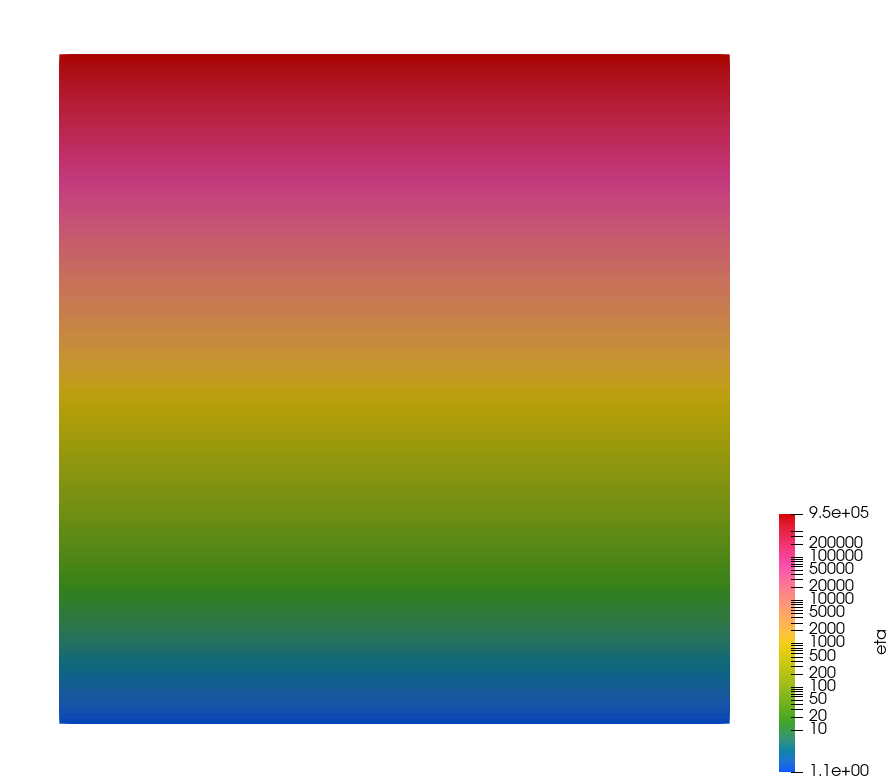
\includegraphics[width=6.5cm]{python_codes/fieldstone_06/results/eta}\\
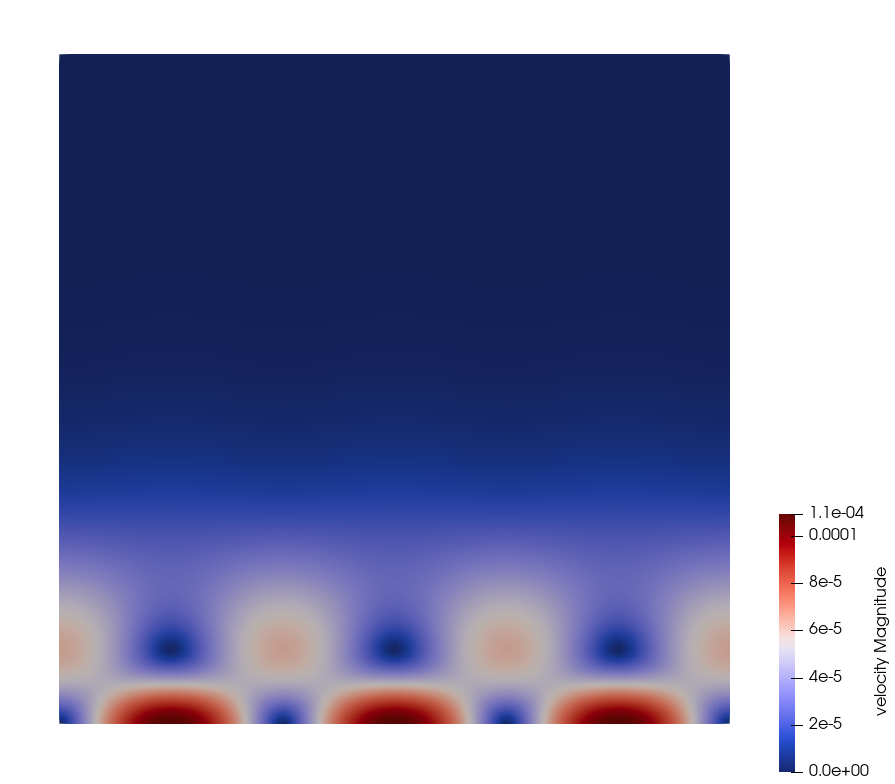
\includegraphics[width=4cm]{python_codes/fieldstone_06/results/vel}
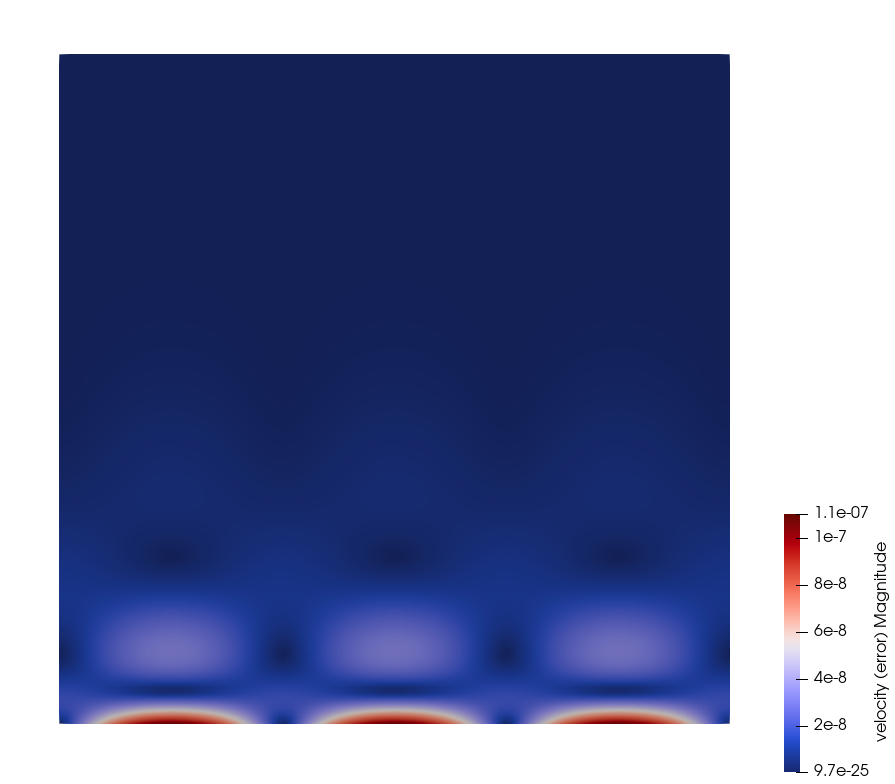
\includegraphics[width=4cm]{python_codes/fieldstone_06/results/vel_error}
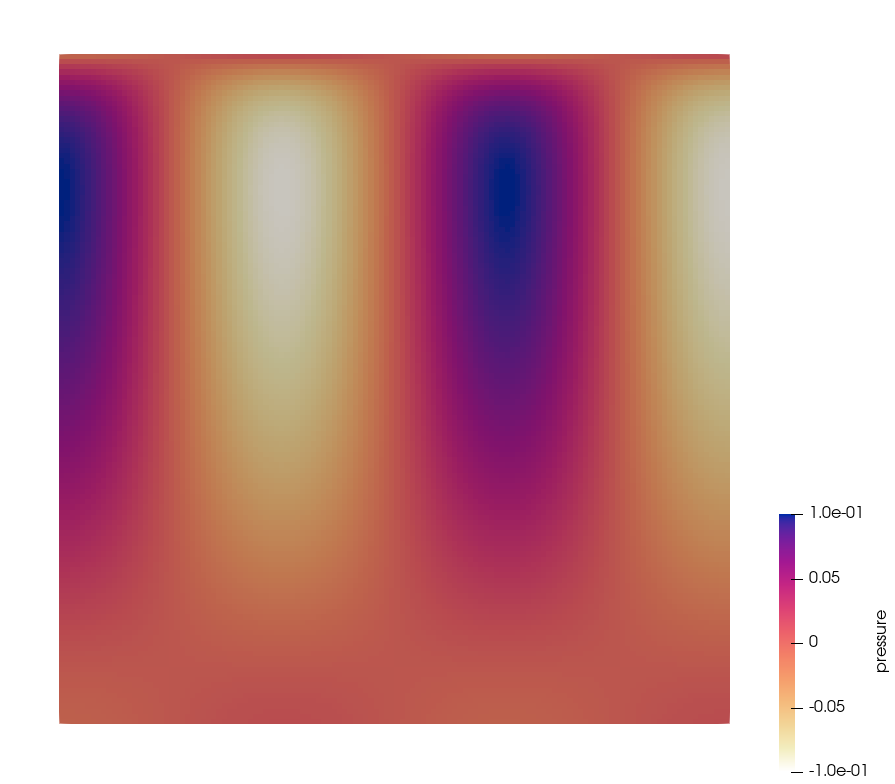
\includegraphics[width=4cm]{python_codes/fieldstone_06/results/press}
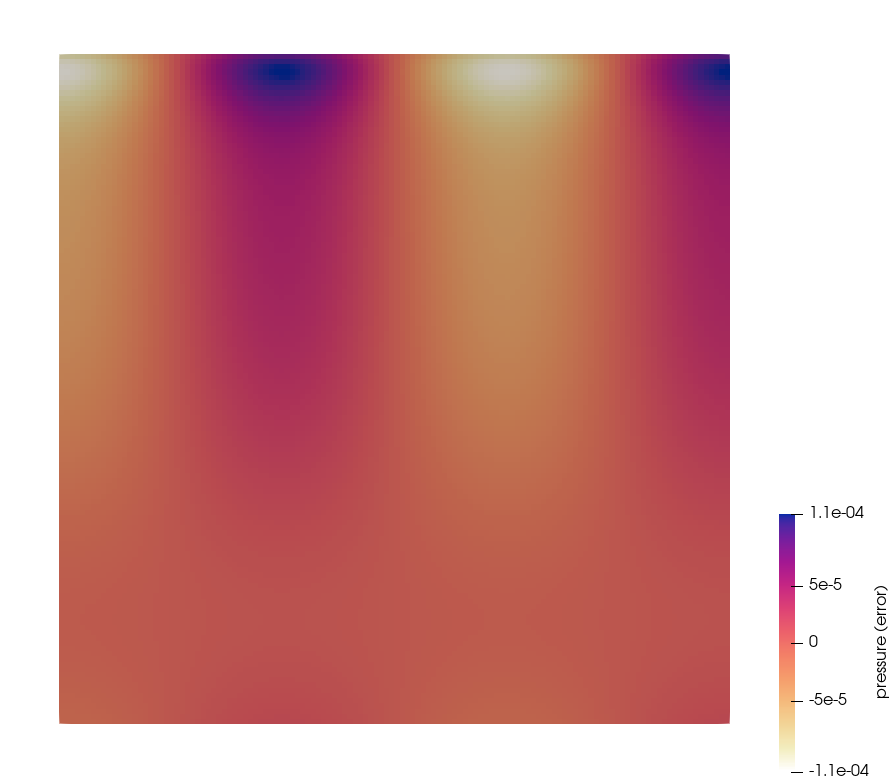
\includegraphics[width=4cm]{python_codes/fieldstone_06/results/press_error}\\
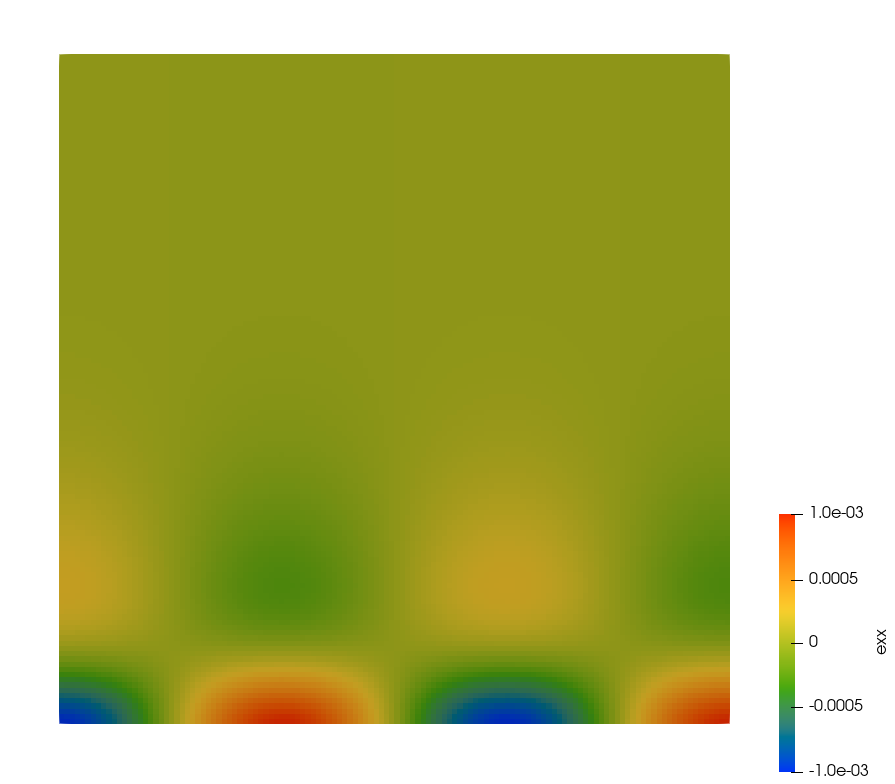
\includegraphics[width=4cm]{python_codes/fieldstone_06/results/exx}
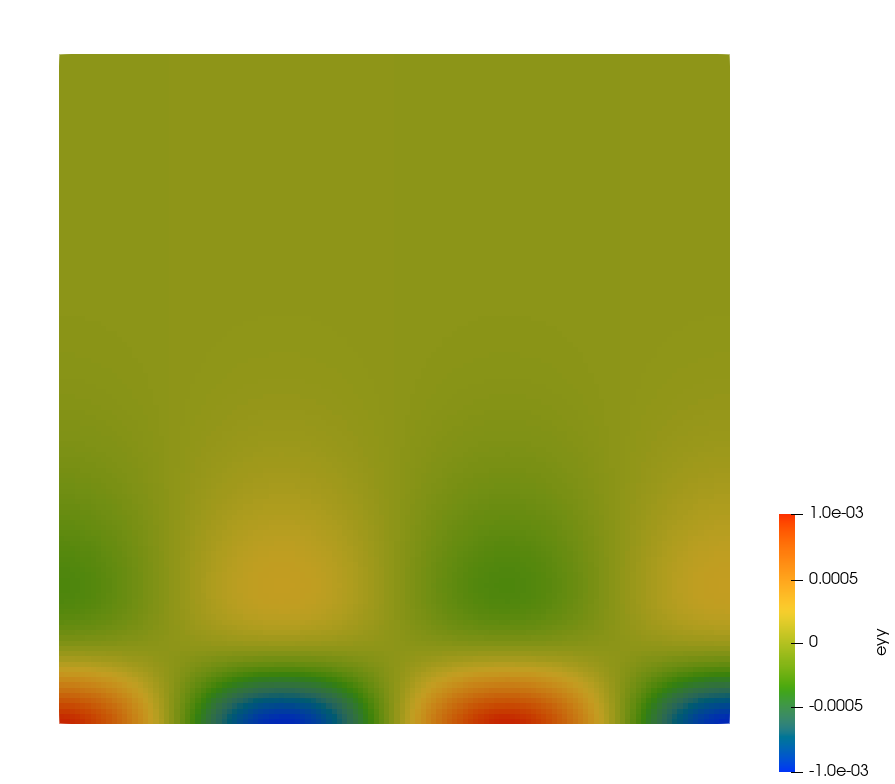
\includegraphics[width=4cm]{python_codes/fieldstone_06/results/eyy}
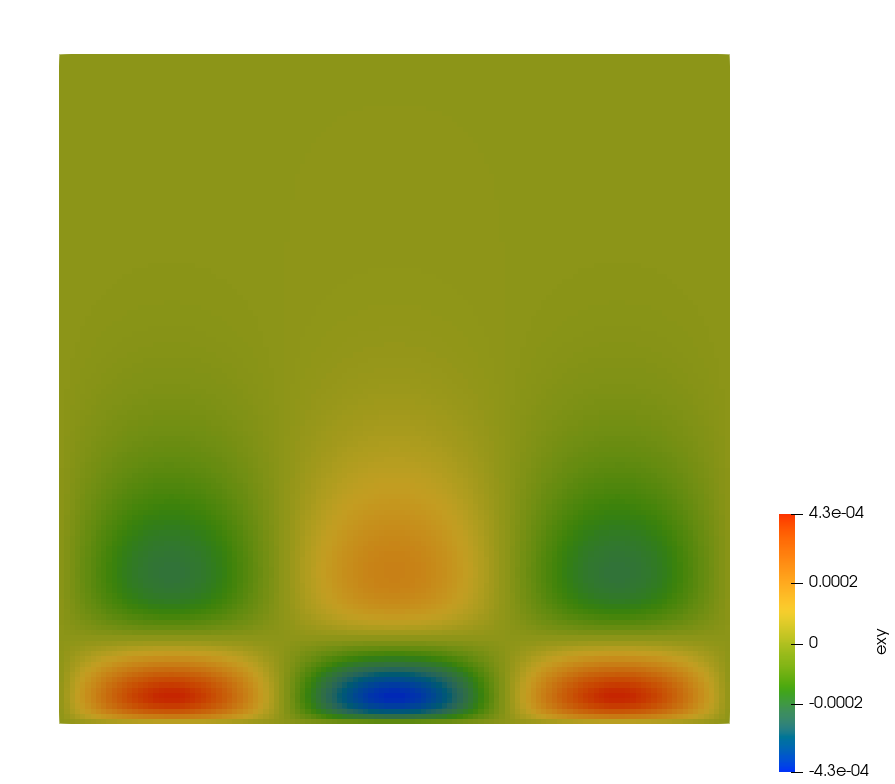
\includegraphics[width=4cm]{python_codes/fieldstone_06/results/exy}
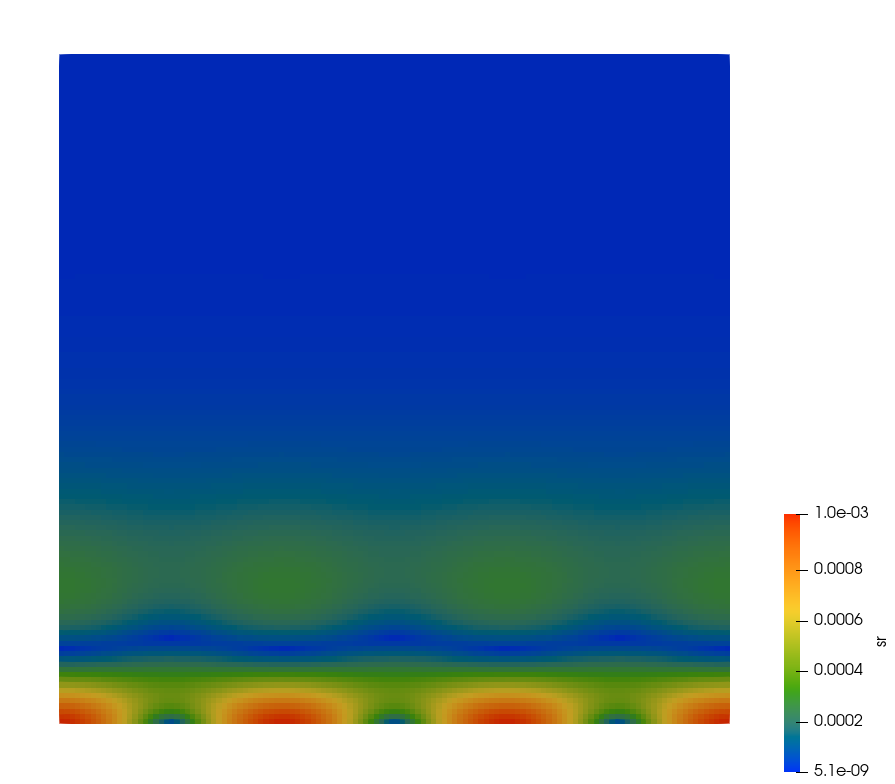
\includegraphics[width=4cm]{python_codes/fieldstone_06/results/sr}\\
{\captionfont Results obtained on $128 \times 128$ mesh.}
\end{center}

We recover a quadratic convergence for the velocity error and 
a linear convergence for the pressure error:

\begin{center}
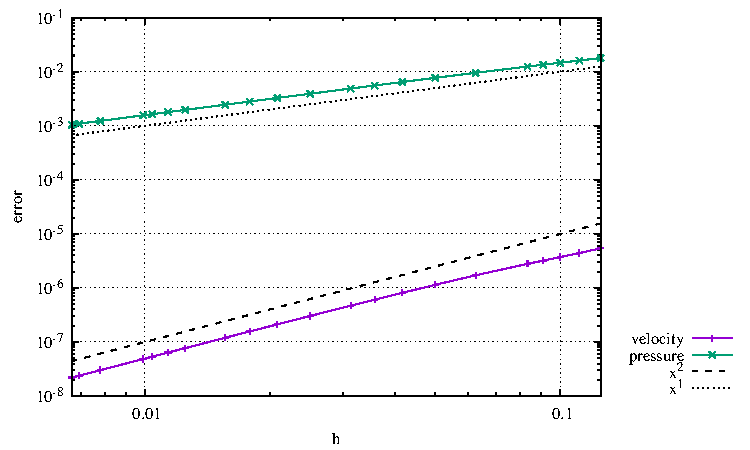
\includegraphics[width=12cm]{python_codes/fieldstone_06/results/errors.pdf}\\
{\captionfont Velocity and pressure error as a function of mesh size.}
\end{center}
